%\setcounter{subsubsection}{0}
\subsubsection{Dao động tắt dần}
\begin{center}
\begin{tikzpicture}[draw=Mapcolor,scale=1,thick,>=stealth']
\tkzDefPoints{0.4/0.5/v}
\draw[->] (0,0)--(8.5,0)node[below]{$t$};
\draw[->] (0,-2.5)--(0,2.5)node[right]{$x$};
\draw[Mapcolor, line width = 1.2pt, domain=0:7.5, samples=500]%
plot (\x, {2*e^(-\x/4)*cos(\x*180)});
\draw[thick,dashed] plot [smooth,tension=1] coordinates{(0,2)(3,1) (7.5,0.3)};
\draw[thick,dashed] plot [smooth,tension=1] coordinates{(0,-2)(3,-1) (7.5,-0.3)};
\end{tikzpicture}
\end{center}
\newghichu{Dao động tắt dần là dao động có biên độ giảm dần theo thời gian.} 
\vspace*{0.2cm}
\begin{itemize}
\item \textbf{Nguyên nhân:} Do vật chuyển động chịu tác dụng của lực ma sát và lực cản của môi trường đó.
\item \textbf{Đặc điểm:}
\begin{itemize}
\item Cơ năng của vật giảm dần và chuyển hóa thành nhiệt năng.
\item Tùy theo lực cản của môi trường lớn hay nhỏ mà dao động tắt dần diễn ra nhanh hay chậm.
\end{itemize}
\end{itemize}


\immini{\begin{itemize}
\item \textbf {Ứng dụng của dao động tắt dần:}
\begin{itemize}
\item  Dao động tắt dần có lợi: Bộ phận giảm xóc trên ô tô, xe máy,\ldots, kiểm tra, thay dầu nhớt.
\item Dao động tắt dần có hại: Dao động tắt dần ở quả lắc đồng hồ $\rightarrow$ phải lên dây cót hoặc thay pin.
\end{itemize}
\end{itemize}}{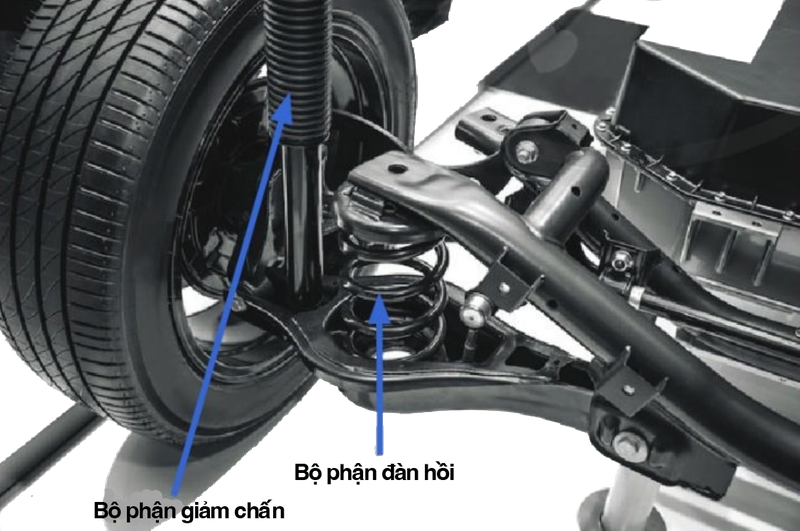
\includegraphics[width=4cm]{Hinh/LTK11-2}}

\immini{\subsubsection{Dao động duy trì}
\newghichu{Dao động duy trì là dao động tắt dần nhưng được bù lại năng lượng tiêu hao sao cho không làm thay đổi chu kì riêng và biên độ của vật.}
\vspace*{0.2cm}
\begin{itemize}
\item \par \textbf{Đặc điểm:}
\begin{itemize}
\item Tần số bằng tần số dao động riêng. 
\item Biên độ không đổi.
\end{itemize}
\end{itemize}}{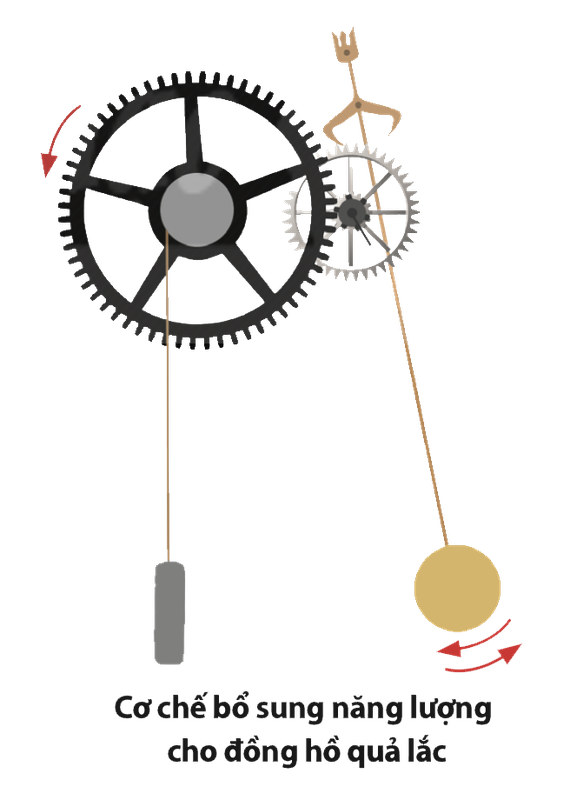
\includegraphics[width=4cm]{Hinh/LTK11}}
\subsubsection{Dao động cưỡng bức}
\immini{
\newghichu{Dao động cưỡng bức là dao động luôn chịu tác dụng của ngoại lực biến thiên tuần hoàn, biểu thức ngoại lực có dạng
\begin{align*}
F=F_0\cos(\omega t+\varphi) 
\end{align*}}}{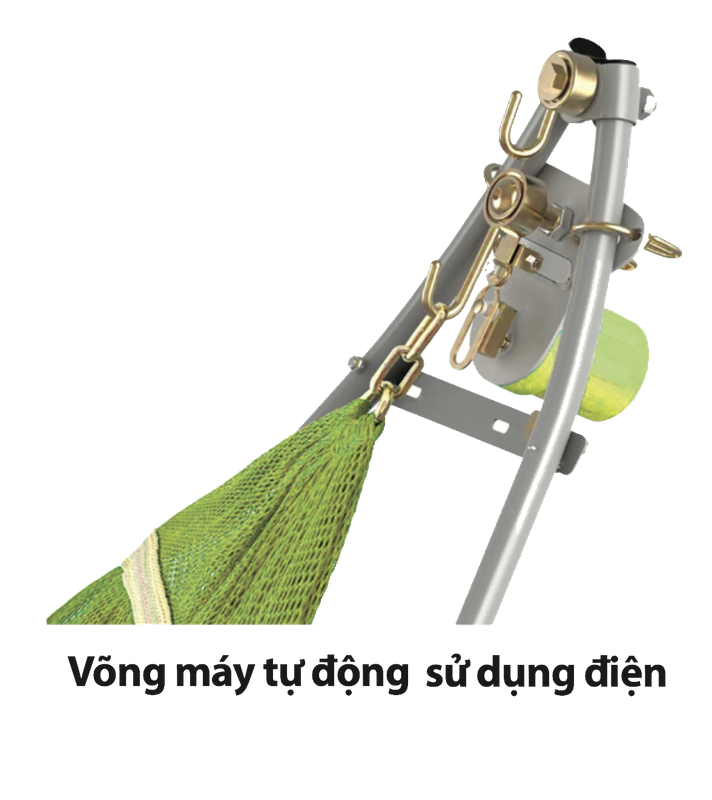
\includegraphics[width=4cm]{Hinh/LTK11-3}}
\begin{itemize}
\item \textbf{Đặc điểm}
\begin{itemize}
\item \textbf{Về tần số}: Trong khoảng thời gian ban đầu nhỏ, dao động của vật là một dao động phức tạp vì đó là sự tổng hợp của dao động riêng và dao động do ngoại lực gây ra. Sau khoảng thời gian nhỏ này, dao động riêng bị tắt hẳn, chỉ còn lại dao động do tác dụng của ngoại lực gây ra, đó là dao động cưỡng bức và dao động cưỡng bức này có tần số đúng bằng tần số của lực cưỡng bức. 
\item \textbf{Về biên độ}: Dao động cưỡng bức có biên độ phụ thuộc vào $F_0$, vào ma sát và đặc biệt phụ thuộc vào độ chênh lệch tần số f của lực cưỡng bức và tần số riêng $f_0$ của hệ. Nếu tần số f càng gần với tần số riêng $f_0$ thì biên độ của dao động cưỡng bức càng tăng và nếu $f = f_0$ thì xảy ra cộng hưởng.
\end{itemize}
\end{itemize}
\immini{\subsubsection{Hiện tượng cộng hưởng}
\newghichu{\textbf{Hiện tượng cộng hưởng} là hiện tượng biên độ của dao động cưỡng bức tăng đến giá trị cực đại khi $f=f_0$ (tần số của ngoại lực bằng tần số riêng của hệ)}}{\begin{tikzpicture}[draw=Mapcolor, very thick,]
%Định nghĩa màu
\definecolor{safetyorange(blazeorange)}{rgb}{1.0, 0.4, 0.0}
\definecolor{royalblue(web)}{rgb}{0.25, 0.41, 0.88}
% Hệ trục
\draw[->] (0,0.4) -- ++(7,0) node [below] {\small Tần số của}node [below=15pt] {\small lực cưỡng bức};
\draw[->] (0.4,0) -- ++(0,6) ;
\node  [left,rotate=90] at (0,4.5){\small Biên độ dao động};
% % Đồ thị
\draw[royalblue(web), very thick] (0.8,0.93) .. controls (2.1,1.63) and (2.66,2.53) .. (3.08,4.14) .. controls (3.49,6.09) and (3.49,6.1) .. (3.88,3.95) .. controls (4.19,2.69) and (4.44,1.49) .. (6.71,0.66);
\draw[safetyorange(blazeorange), very thick](0.78,0.86) .. controls (2.05,1.2) and (2.72,2.41) .. (3.08,3.14) .. controls (3.42,3.82) and (3.58,3.7) .. (3.88,2.95) .. controls (4.42,1.56) and (5.26,1.06) .. (6.74,0.57);
\draw[red!70!black, very thick](0.8,0.81) .. controls (1.97,0.99) and (2.56,1.57) .. (3,1.97) .. controls (3.32,2.24) and (3.51,2.45) .. (3.88,2.03) .. controls (4.39,1.45) and (5.31,0.83) .. (6.68,0.53);

% 
%Chú thích
\draw[dashed] (3.49,0.4) -- ++(0,5.2) node [pos=-0.05] {\small$f_0$}node [pos=-0.15] {\small (Tần số riêng)};
\draw (4.8,4.8) -- (4,3.5) node [pos=-0.2] {\scriptsize Lực cản nhỏ};
\draw (5,2.3) -- (4.06,1.85) node [pos=0.1, above right] {\scriptsize Lực cản lớn};
\end{tikzpicture}}
\subsubsection{Ứng dụng của hiện tượng cộng hưởng}
\begin{itemize}
\item \textbf{Ưu điểm:} Hiện tượng cộng hưởng có nhiều ứng dụng trong thực tế, ví dụ: chế tạo tần số kế, lên dây đàn, đóng thùng loa,\ldots
\item \textbf{Nhược điểm:} 
\begin{itemize}
\item Mỗi một bộ phận trong máy móc (hoặc cầu cống) đều có thể xem là một hệ dao động có tần số góc $\omega_0$ riêng.
\item Khi thiết kế các bộ phận của máy móc cần chú ý đến sự trùng nhau giữa tần số góc $\omega$ của ngoại lực và tần số góc $\omega_0$ riêng của các bộ phận này, nếu các bộ phận này dao động trùng nhau về tần số góc thì có thể xảy ra ra hiện tượng cộng hưởng với biên độ rất lớn và có thể làm gãy, vỡ các chi tiết máy móc.
\end{itemize}
\begin{center}
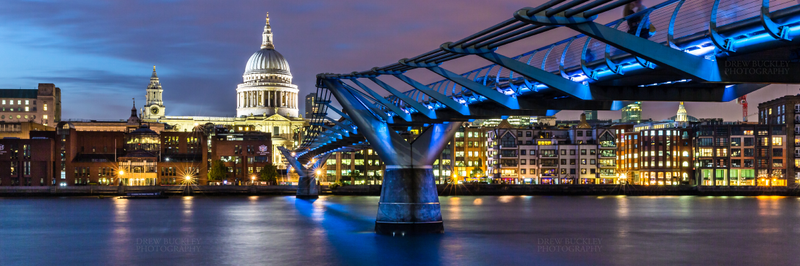
\includegraphics[width=14cm]{Hinh/LTK11-4}
\end{center}
\end{itemize}
